	% Darmstadt|Frankfurt|JuanLesPins
	
	\documentclass{beamer}
	\setbeamertemplate{navigation symbols}{}
	
	\usetheme{hpi}
	\usepackage[ngerman]{babel}
	\usepackage[utf8]{inputenc}
	\usepackage{geometry}
	\usepackage[T1]{fontenc}
	\usepackage{graphicx} %Zum Bilder einbinden
	\usepackage{float} %Damit die Figures, also die Bilder, mitten im Text, an geforceter Position erscheinen
	\usepackage{verbatim} %für mehrzeilige Kommentare \begin~\end{comment}
	\usepackage{amstext} % \text{asdf} in Formeln, statt \mbox, weil mbox die Schriftgröße festsetzt	
	\usepackage{amsmath}
	\usepackage{amssymb}
	\usepackage{ucs}
	\usepackage{BeamerColor}
	
	\usepackage{listings}
	\usepackage{color}
	\usepackage{hyperref}
	\usepackage{acronym}
	\definecolor{tplcolor}{HTML}{F6AE15}
	\usecolortheme[named=tplcolor]{structure}
	
	\lstset{
		language=Java, 
		inputencoding=utf8,
		tabsize=2,
		basicstyle=\tiny,
		captionpos=b,language=JAVA,breaklines=true,      % the size of the fonts that are used for the line-numbers,
		stepnumber=5,   
		keywordstyle=\color{brown},
		commentstyle=\color{DarkGreen}, 
		stringstyle=\color{blue},
		showstringspaces=false,
		breaklines=true
		literate=%
		{Ö}{{\"O}}1
		{Ä}{{\"A}}1
		{Ü}{{\"U}}1
		{ß}{{\ss}}1
		{ü}{{\"u}}1
		{ä}{{\"a}}1
		{ö}{{\"o}}1
		{~}{{\textasciitilde}}1	
	}

	\beamersetuncovermixins{\opaqueness<1>{25}}{\opaqueness<2->{15}}
	
	\usecaptiontemplate{
	\tiny
	\structure{\insertcaptionname~\insertcaptionnumber:}
	\insertcaption
	}
	
	\usefootnotetemplate{
	\tiny
	\parindent 1em\noindent
	\hbox to 1.8em{\hfil\insertfootnotemark}\insertfootnotetext
	}
	\begin{document}
			
	\setbeamercovered{invisible}
	
	\title[Review - Entwurfsprojekt]{Review - Entwurfsprojekt\\ Eine Logistiksoftware für MöbelCorp}
	\author{Gruppe 3}
	
	 \begin{frame}[title=Hauptgebaeude_Nacht.jpg]
	 	\maketitle
	 	\date{26. Mai 2018}
 	\end{frame}
	 
	\begin{frame}
		\frametitle{Gliederung}
		\tableofcontents
		%Folien mit einem * im Titel sollen beim Vortrag übersprungen werden.
	\end{frame}
	\section{Abstrakte Architektur}
	\begin{frame}{Abstrakte Architektur}
		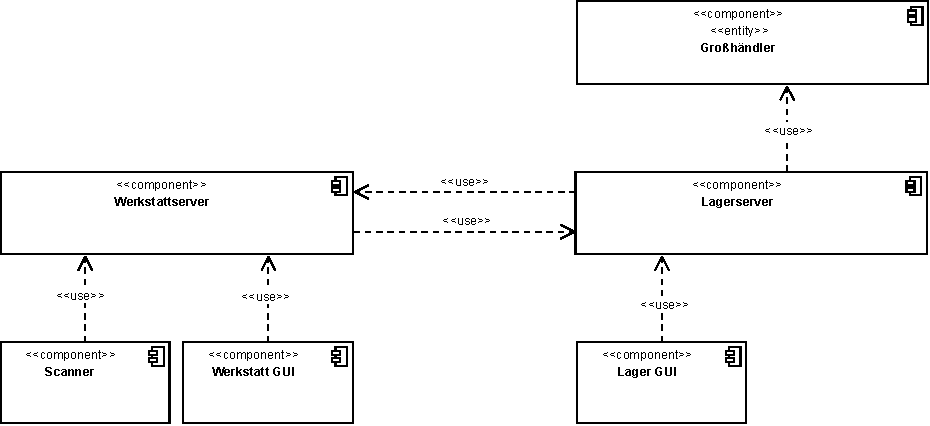
\includegraphics[width=\textwidth]{PDF/abstrakte_Architektur.pdf}
	\end{frame}
	\section{Interaktion der Komponenten}
	\begin{frame}{Interaktion der Komponenten}

	\end{frame}
	\section{Komponentenschnittstellen}
	\begin{frame}{Komponentenschnittstellen}

	\end{frame}
	\section{Konkrete Architektur}
	\begin{frame}{Konkrete Architektur}

	\end{frame}
	\section{ Innere Struktur der Komponenten}
	\begin{frame}{Innere Struktur der Komponenten}

	\end{frame}
	\section{Paketstruktur}
	\begin{frame}{Paketstruktur}

	\end{frame}
	\section{Paketdetails}
	\begin{frame}{Paketdetails}

	\end{frame}

	\begin{frame}[title=Hauptgebaeude_Nacht.jpg]
		\maketitle
		\date{26. Mai 2018}
	\end{frame}
\end{document}

